\documentclass[aspectratio=169,11pt]{beamer}
\usepackage[utf8]{inputenc}
\usepackage[T1]{fontenc}
\usepackage{graphicx}
\usepackage{booktabs}
\usepackage[table]{xcolor}
\usepackage{amsmath}
\usepackage{listings}
\usepackage{tikz}
\usetikzlibrary{arrows.meta,positioning,fit,shapes.geometric}

%% ---- Theme ----
\usetheme{Madrid}
\usecolortheme{default}
\definecolor{myblue}{RGB}{31,78,121}
\definecolor{myred}{RGB}{192,0,0}
\definecolor{mygreen}{RGB}{0,112,44}
\setbeamercolor{structure}{fg=myblue}
\setbeamercolor{frametitle}{bg=myblue,fg=white}
\setbeamercolor{title}{bg=myblue,fg=white}
\setbeamercolor{block title}{bg=myblue!80,fg=white}
\setbeamercolor{alerted text}{fg=myred}
\setbeamerfont{frametitle}{series=\bfseries}

\lstset{
    basicstyle=\ttfamily\scriptsize,
    backgroundcolor=\color{myblue!5},
    frame=single, rulecolor=\color{myblue!30},
    breaklines=true, xleftmargin=4pt, xrightmargin=4pt
}

%% ---- Meta ----
\title[Adversarially Robust IDS]{Adversarially Robust\\Intrusion Detection System}
\subtitle{Deep Learning en Cybers\'ecurit\'e --- Projet 1}
\author{Zakariya El Mansouri}
\institute{ICCN-INE2}
\date{Avril 2026}

%% ---- Footer ----
\setbeamertemplate{footline}{
  \leavevmode\hbox{%
  \begin{beamercolorbox}[wd=.33\paperwidth,ht=2.25ex,dp=1ex,center]{author in head/foot}%
    \usebeamerfont{author in head/foot}\insertshortauthor
  \end{beamercolorbox}%
  \begin{beamercolorbox}[wd=.34\paperwidth,ht=2.25ex,dp=1ex,center]{title in head/foot}%
    \usebeamerfont{title in head/foot}\insertshorttitle
  \end{beamercolorbox}%
  \begin{beamercolorbox}[wd=.33\paperwidth,ht=2.25ex,dp=1ex,right]{date in head/foot}%
    \usebeamerfont{date in head/foot}\insertframenumber{} / \inserttotalframenumber\hspace*{2ex}
  \end{beamercolorbox}}%
  \vskip0pt%
}

\begin{document}

%% ============================================================
%% TITLE
%% ============================================================
\begin{frame}
\titlepage
\end{frame}

%% ============================================================
%% PLAN
%% ============================================================
\begin{frame}{Plan}
\tableofcontents
\end{frame}

%% ============================================================
\section{Contexte et Threat Model}
%% ============================================================

\begin{frame}{Probl\'ematique}
\begin{columns}[T]
\column{0.55\textwidth}
\begin{block}{Syst\`eme de D\'etection d'Intrusion (IDS)}
\begin{itemize}
    \item Surveille le trafic r\'eseau
    \item D\'etecte les connexions malveillantes
    \item Base\'e sur l'apprentissage automatique
\end{itemize}
\end{block}
\vspace{0.4em}
\begin{alertblock}{Probl\`eme : exemples adversariaux}
Un attaquant peut modifier l\'eg\`erement son trafic pour \alert{tromper le mod\`ele} tout en maintenant l'efficacit\'e de l'attaque.
\end{alertblock}

\column{0.42\textwidth}
\begin{center}
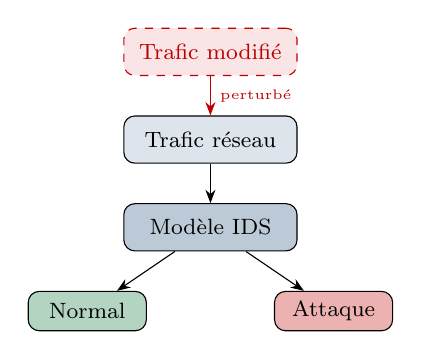
\begin{tikzpicture}[scale=0.85, every node/.style={font=\footnotesize}]
  \node[draw,rounded corners,fill=myblue!15,minimum width=2.2cm,minimum height=0.6cm] (traffic) {Trafic r\'eseau};
  \node[draw,rounded corners,fill=myblue!30,minimum width=2.2cm,minimum height=0.6cm, below=0.5cm of traffic] (ids) {Mod\`ele IDS};
  \node[draw,rounded corners,fill=mygreen!30,minimum width=1.5cm,minimum height=0.5cm, below left=0.5cm and -0.3cm of ids] (norm) {Normal};
  \node[draw,rounded corners,fill=myred!30,minimum width=1.5cm,minimum height=0.5cm, below right=0.5cm and -0.3cm of ids] (atk) {Attaque};
  \draw[-{Stealth}] (traffic) -- (ids);
  \draw[-{Stealth}] (ids) -- (norm);
  \draw[-{Stealth}] (ids) -- (atk);
  \node[draw,dashed,myred,rounded corners,fill=myred!10,minimum width=2.2cm,minimum height=0.6cm, above=0.5cm of traffic] (adv) {\alert{Trafic modifi\'e}};
  \draw[-{Stealth},myred] (adv) -- node[right,font=\tiny]{perturb\'e} (traffic);
\end{tikzpicture}
\end{center}
\end{columns}
\end{frame}

\begin{frame}{Threat Model}
\begin{columns}[T]
\column{0.48\textwidth}
\begin{block}{\checkmark\ Features manipulables (14/42)}
L'attaquant contr\^ole le timing et le volume :
\medskip

\texttt{\footnotesize dur, spkts, dpkts, sbytes, dbytes,\\
sttl, sload, dload, sinpkt, dinpkt,\\
sjit, djit, smean, dmean}
\end{block}

\column{0.48\textwidth}
\begin{alertblock}{\texttimes\ Features non manipulables}
Changer ces valeurs briserait l'attaque :
\medskip

\texttt{\footnotesize proto, service, state,\\srcip, dstip, dport}
\end{alertblock}
\end{columns}

\vspace{0.8em}
\begin{exampleblock}{Mod\`ele de l'attaquant}
\begin{itemize}
    \item \textbf{White-box} : acc\`es complet au mod\`ele (gradients disponibles)
    \item \textbf{Objectif} : faire classer une attaque comme trafic normal (\emph{evasion})
    \item \textbf{Budget} : perturbation born\'ee par $\varepsilon$ en norme $\ell_\infty$
\end{itemize}
\end{exampleblock}
\end{frame}

%% ============================================================
\section{Dataset et Pr\'etraitement}
%% ============================================================

\begin{frame}{Dataset UNSW-NB15}
\begin{columns}[T]
\column{0.52\textwidth}
\begin{block}{Caract\'eristiques}
\begin{itemize}
    \item Trafic r\'eseau r\'eel captur\'e en laboratoire
    \item 9 types d'attaques (DoS, Exploits, Backdoors, ...)
    \item \textbf{42 features} par connexion
\end{itemize}
\end{block}

\begin{table}
\footnotesize
\begin{tabular}{lrr}
\toprule
\textbf{Ensemble} & \textbf{Exemples} & \textbf{Attaques} \\
\midrule
Train & 82\,332  & 55.1\% \\
Test  & 175\,341 & --- \\
\bottomrule
\end{tabular}
\end{table}

Classes bien \'equilibr\'ees $\Rightarrow$ pas de biais.

\column{0.46\textwidth}
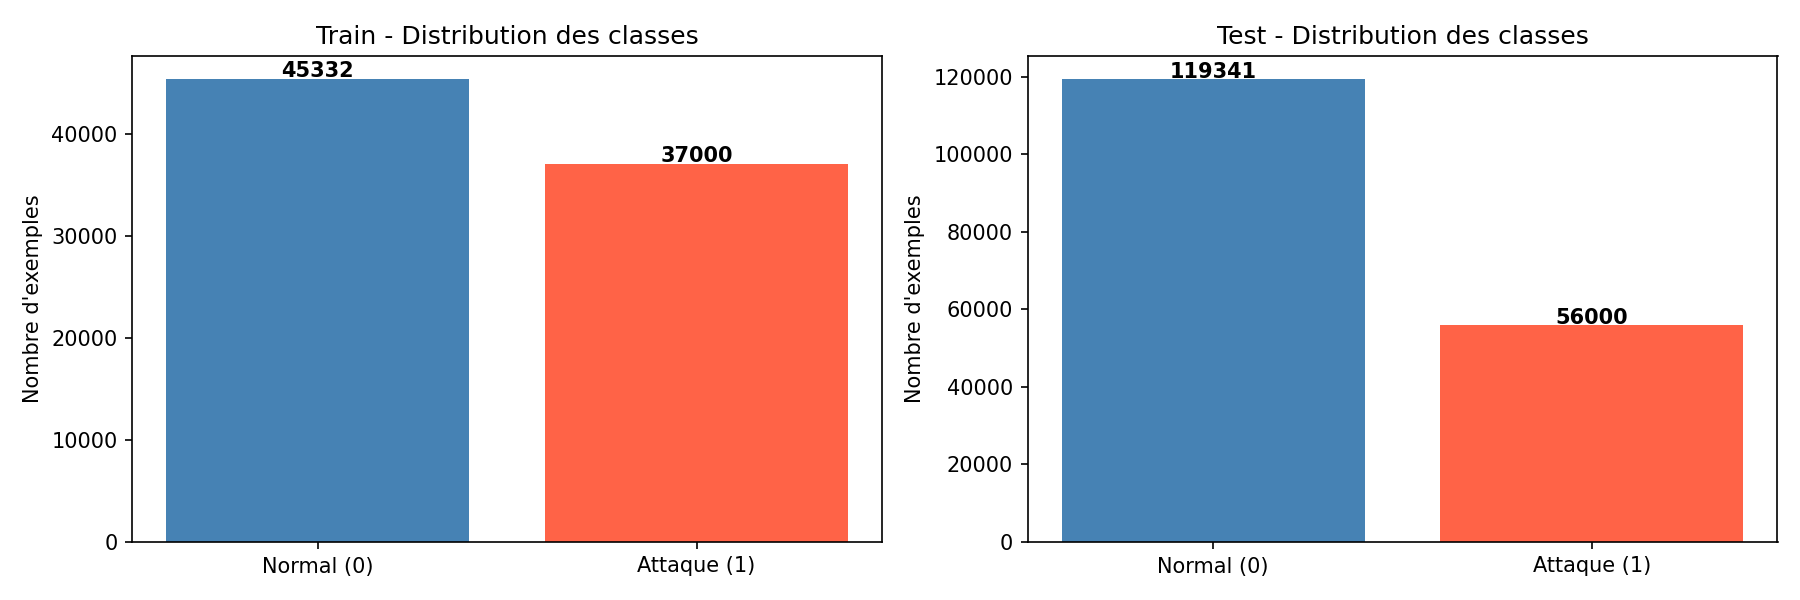
\includegraphics[width=\textwidth]{../results/class_distribution.png}
\end{columns}
\end{frame}

\begin{frame}{Pipeline de Pr\'etraitement}
\begin{center}
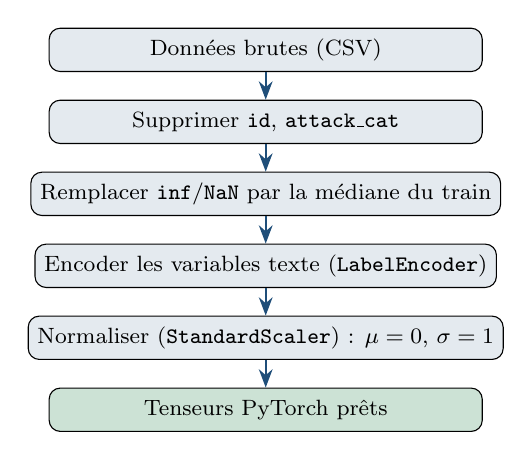
\begin{tikzpicture}[
    node distance=0.35cm,
    box/.style={draw,rounded corners,fill=myblue!12,minimum width=5.5cm,minimum height=0.55cm,font=\footnotesize,align=center},
    arr/.style={-{Stealth},myblue,thick}
]
\node[box] (raw)  {Donn\'ees brutes (CSV)};
\node[box,below=of raw] (drop) {Supprimer \texttt{id}, \texttt{attack\_cat}};
\node[box,below=of drop] (nan)  {Remplacer \texttt{inf}/\texttt{NaN} par la m\'ediane du train};
\node[box,below=of nan]  (enc)  {Encoder les variables texte (\texttt{LabelEncoder})};
\node[box,below=of enc]  (sc)   {Normaliser (\texttt{StandardScaler}) : $\mu=0$, $\sigma=1$};
\node[box,below=of sc,fill=mygreen!20]   (ok)   {Tenseurs PyTorch pr\^ets};
\foreach \a/\b in {raw/drop,drop/nan,nan/enc,enc/sc,sc/ok}
    \draw[arr] (\a) -- (\b);
\end{tikzpicture}
\end{center}
\vspace{0.2em}
\footnotesize \textbf{Pourquoi normaliser ?} Sans normalisation, \texttt{sbytes} $\in [0, 10^6]$ \'ecrase \texttt{sttl} $\in [0,255]$.
\end{frame}

%% ============================================================
\section{Mod\`ele Baseline}
%% ============================================================

\begin{frame}{Architecture MLP}
\begin{columns}[T]
\column{0.55\textwidth}
\[
\underbrace{42}_{\text{input}}
\!\xrightarrow{+\text{ReLU}+\text{Drop}}\! 128
\!\xrightarrow{+\text{ReLU}+\text{Drop}}\! 64
\!\xrightarrow{+\text{ReLU}}\! 32
\!\xrightarrow{+\sigma}\! 1
\]

\vspace{0.4em}
\begin{itemize}
    \item \textbf{Dropout 0.3} : \'eteint 30\% des neurones al\'eatoirement $\Rightarrow$ anti-surapprentissage
    \item \textbf{Sigmoid} : sortie $\in [0,1]$, seuil 0.5
    \item Optimiseur Adam, $lr=10^{-3}$, BCE Loss
    \item 30 epochs, batch 512
\end{itemize}

\column{0.43\textwidth}
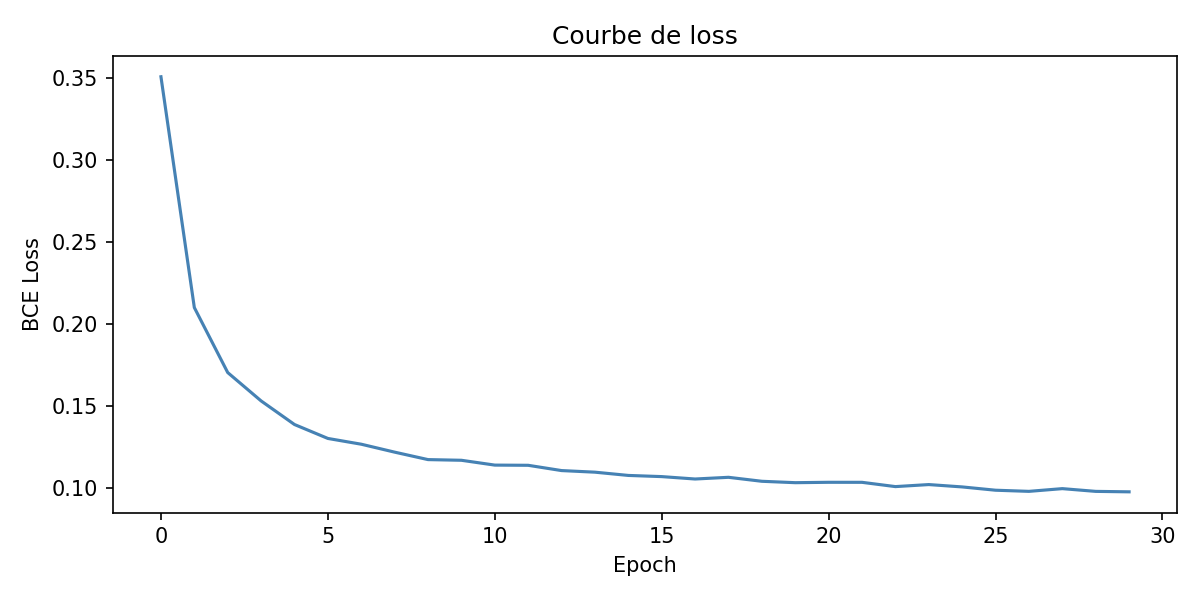
\includegraphics[width=\textwidth]{../results/training_loss.png}
\end{columns}
\end{frame}

\begin{frame}{R\'esultats Baseline}
\begin{columns}[T]
\column{0.45\textwidth}
\begin{block}{M\'etriques sur donn\'ees propres}
\begin{tabular}{lr}
\toprule
F1-score   & \textbf{0.9110} \\
Precision  & 0.9879 \\
Recall     & 0.8452 \\
PR-AUC     & 0.9881 \\
\midrule
\rowcolor{myred!15}
Evasion Rate & 15.5\% \\
\bottomrule
\end{tabular}
\end{block}
\vspace{0.3em}
\alert{15.5\%} des attaques passent d\'ej\`a sans modification~!

\column{0.52\textwidth}
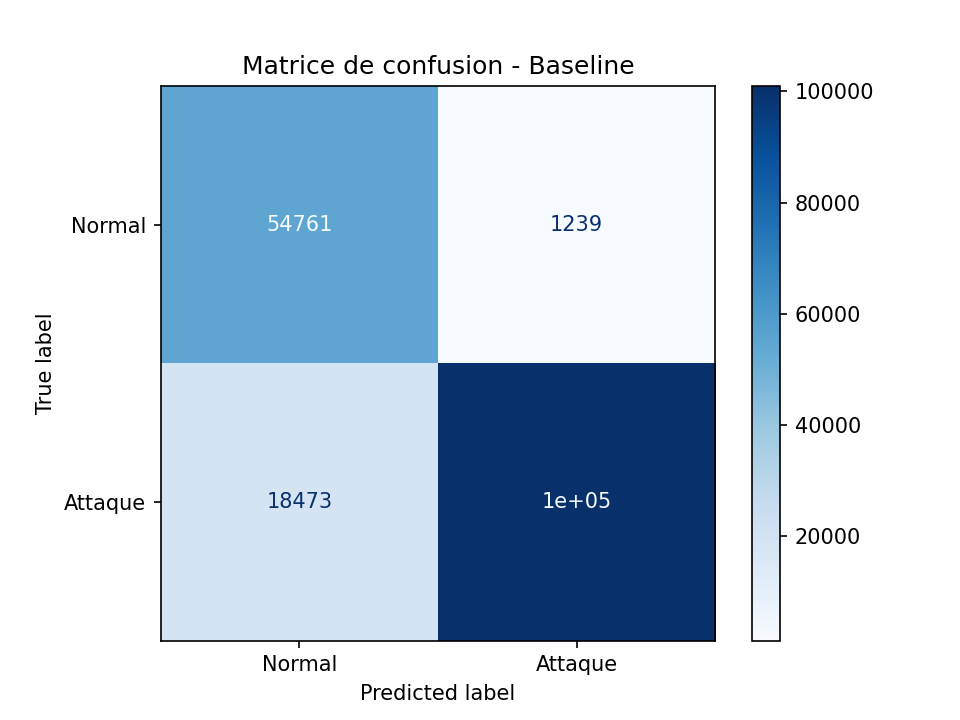
\includegraphics[width=\textwidth]{../results/confusion_baseline.png}
\end{columns}
\end{frame}

%% ============================================================
\section{Attaques Adversariales}
%% ============================================================

\begin{frame}{FGSM --- Fast Gradient Sign Method}
\begin{block}{Formule}
\[
X_{\text{adv}} = X + \varepsilon \cdot \underbrace{\text{sign}\!\left(\nabla_X \mathcal{L}(f(X), y)\right)}_{\text{direction qui maximise l'erreur}} \cdot \underbrace{\mathbf{m}}_{\text{masque manipulable}}
\]
\end{block}

\begin{columns}[T]
\column{0.54\textwidth}
\textbf{Algorithme :}
\begin{enumerate}
    \item Calculer la perte BCE sur l'exemple d'attaque
    \item Backpropagate $\Rightarrow$ gradient des features
    \item Perturber dans la direction du gradient
    \item Appliquer uniquement sur les 14 features manipulables
\end{enumerate}

\column{0.43\textwidth}
\begin{exampleblock}{Intuition}
Le gradient dit \textit{``si tu augmentes cette feature, le mod\`ele se trompe davantage''}.
On l'augmente de exactement $\varepsilon$.
\end{exampleblock}
\end{columns}
\end{frame}

\begin{frame}{PGD --- Projected Gradient Descent}
\begin{block}{Formule}
\[
X^{(t+1)} = \Pi_{B(X,\varepsilon)}\!\left[X^{(t)} + \alpha \cdot \text{sign}\!\left(\nabla_{X^{(t)}} \mathcal{L}\right) \cdot \mathbf{m}\right],\quad \alpha = \frac{\varepsilon}{T}
\]
\end{block}

\begin{columns}[T]
\column{0.54\textwidth}
\begin{itemize}
    \item FGSM it\'er\'e ($T=10$ \'etapes)
    \item Apr\`es chaque pas, \textbf{projection} dans la boule $\ell_\infty$ de rayon $\varepsilon$
    \item Explore plus finement l'espace de perturbation
    \item \alert{Attaque de r\'ef\'erence} pour \'evaluer la robustesse
\end{itemize}

\column{0.43\textwidth}
\begin{alertblock}{PGD > FGSM}
FGSM fait un grand pas aveugle.\\PGD fait 10 petits pas adapt\'es.
\end{alertblock}
\end{columns}
\end{frame}

\begin{frame}{R\'esultats des Attaques ($\varepsilon = 0.1$)}
\begin{columns}[T]
\column{0.55\textwidth}
\begin{table}
\footnotesize
\begin{tabular}{lrrr}
\toprule
\textbf{Sc\'enario} & \textbf{F1} & \textbf{Recall} & \textbf{Evasion\%} \\
\midrule
Propres & 0.9110 & 0.845 & 15.5\% \\
FGSM    & 0.8533 & 0.752 & 24.8\% \\
\rowcolor{myred!20}
PGD     & 0.8402 & 0.732 & \textbf{26.8\%} \\
\bottomrule
\end{tabular}
\end{table}

\vspace{0.4em}
\begin{alertblock}{Conclusion}
Sous PGD, \alert{1 attaque sur 4} passe inaper\c{c}ue. La pr\'ecision reste \'elev\'ee : les perturbations ne cr\'eent pas de faux positifs, elles font juste \'evader des vraies attaques.
\end{alertblock}

\column{0.42\textwidth}
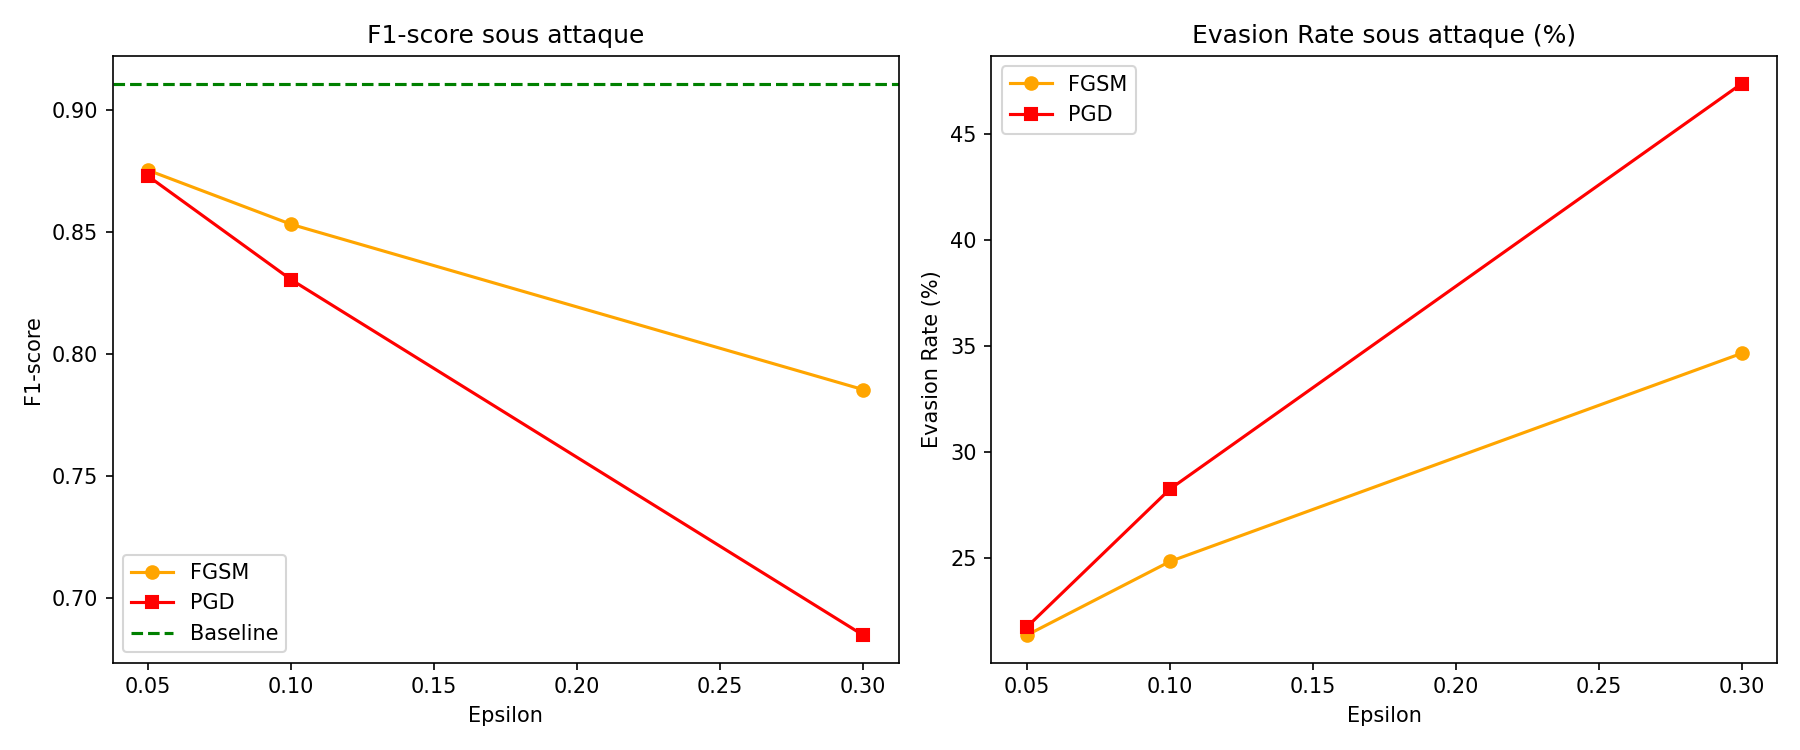
\includegraphics[width=\textwidth]{../results/attack_comparison.png}
\end{columns}
\end{frame}

%% ============================================================
\section{D\'efenses}
%% ============================================================

\begin{frame}{D\'efense 1 --- Adversarial Training : Approche 1 (FGSM-AT)}
\begin{columns}[T]
\column{0.54\textwidth}
\begin{block}{Principe}
Re-entra\^iner sur un mix 50\% propres + 50\% FGSM.
\end{block}
\vspace{0.3em}
\textbf{R\'esultat :}
\begin{table}
\scriptsize
\begin{tabular}{lrr}
\toprule
Sc\'enario & F1 & Evasion\% \\
\midrule
Propres & 0.8971 & 17.8\% \\
\rowcolor{myred!20}
PGD & 0.7700 & \alert{36.7\%} \\
\bottomrule
\end{tabular}
\end{table}

\alert{Pire que le baseline (28.2\%) !}

\column{0.43\textwidth}
\begin{alertblock}{3 raisons de l'\'echec}
\begin{enumerate}
\scriptsize
    \item \textbf{Robustness gap} : entra\^in\'e FGSM, \'evalu\'e PGD
    \item \textbf{Distribution shift} : mix 50/50 contradictoire
    \item \textbf{Attaque non-stabilis\'ee} : FGSM sur mod\`ele non-converg\'e
\end{enumerate}
\end{alertblock}
\end{columns}
\end{frame}

\begin{frame}{D\'efense 1 --- Adversarial Training : Approche 2 (PGD-AT)}
\begin{columns}[T]
\column{0.54\textwidth}
\begin{block}{Corrections appliqu\'ees}
\begin{itemize}
    \item FGSM $\rightarrow$ \textbf{PGD-7} (m\^eme famille que l'\'evaluation)
    \item 100\% adversarial (\'elimination du distribution shift)
\end{itemize}
\end{block}
\vspace{0.2em}
\[
\min_\theta\; \mathbb{E}\!\left[\max_{\|\delta\|_\infty \leq \varepsilon} \mathcal{L}(f_\theta(x+\delta), y)\right]
\]
\textbf{R\'esultat :}
\begin{table}
\scriptsize
\begin{tabular}{lrr}
\toprule
Sc\'enario & F1 & Evasion\% \\
\midrule
Propres & 0.8943 & 18.1\% \\
\rowcolor{myred!30}
PGD & 0.7425 & \alert{40.2\%} \\
\bottomrule
\end{tabular}
\end{table}

\column{0.43\textwidth}
\begin{alertblock}{Encore pire !}
Entra\^iner sur 100\% PGD sans donn\'ees propres provoque un \textbf{oubli catastrophique}.

\medskip
Le mod\`ele surfit PGD-7 sans g\'en\'eraliser \`a PGD-40.
\end{alertblock}
\vspace{0.3em}
\begin{block}{Conclusion}
L'adversarial training \'echoue sur ce dataset tabulaire h\'et\'erog\`ene.
\end{block}
\end{columns}
\end{frame}

\begin{frame}{D\'efense 1 --- Adversarial Training : Approche 3 (PGD-AT Corrig\'e)}
\begin{columns}[T]
\column{0.54\textwidth}
\begin{block}{Hypoth\`ese}
Combiner PGD-10 (corrige robustness gap) + mix 50/50 (corrige l'oubli catastrophique).
\end{block}
\vspace{0.2em}
Param\`etres : $\varepsilon=0.1$, $\alpha=0.01$, PGD-10, 30 epochs, batch 256, $lr=0.0005$

\vspace{0.3em}
\textbf{R\'esultat :}
\begin{table}
\scriptsize
\begin{tabular}{lrr}
\toprule
Sc\'enario & F1 & Evasion\% \\
\midrule
Propres & 0.9116 & 15.3\% \\
\rowcolor{myred!30}
PGD & 0.7327 & \alert{41.5\%} \\
\bottomrule
\end{tabular}
\end{table}
\alert{Le pire r\'esultat de toutes les approches !}

\column{0.43\textwidth}
\begin{alertblock}{Gradient Masking}
PGD-10 pousse la Sigmoid vers des valeurs tr\`es confiantes (0 ou 1) $\Rightarrow$ gradients faibles.

\medskip
PGD-10 ne trouve plus de perturbation (fausse robustesse), mais PGD-40 contourne en explorant davantage.
\end{alertblock}
\vspace{0.3em}
\begin{block}{Bilan adv. training}
Les 3 variantes \'echouent. La cause : donn\'ees tabulaires h\'et\'erog\`enes, sans structure spatiale.
\end{block}
\end{columns}
\end{frame}

\begin{frame}{D\'efense 2 --- Feature Squeezing}
\begin{columns}[T]
\column{0.54\textwidth}
\begin{block}{Principe}
R\'eduire la pr\'ecision num\'erique pour effacer les petites perturbations \textbf{avant le mod\`ele}.
\end{block}

\[
X_{\text{sq}} = \frac{\left\lfloor \dfrac{X}{X_{\max}} \cdot 2^b + 0.5 \right\rfloor}{2^b} \cdot X_{\max}
\]

Avec $b = 4$ bits $\Rightarrow$ \textbf{16 niveaux} de quantification.

\vspace{0.4em}
\textbf{Avant :} \texttt{dur = 2.10183746} \\
\textbf{Apr\`es :} \texttt{dur = 2.09375} \\[0.2em]
La perturbation tombe dans le m\^eme niveau $\Rightarrow$ effac\'ee.

\column{0.43\textwidth}
\begin{exampleblock}{Pourquoi \c{c}a marche}
L'attaquant calcule sa perturbation en float32 ($\varepsilon \approx 10^{-2}$).
Apr\`es quantification \`a 4 bits, cette pr\'ecision est perdue.
\end{exampleblock}

\begin{block}{Avantage}
\begin{itemize}
    \item Pas de re-entra\^inement
    \item Appliqu\'e \`a l'inf\'erence seulement
    \item Compl\'ementaire \`a tout mod\`ele
\end{itemize}
\end{block}
\end{columns}
\end{frame}

%% ============================================================
\section{Comparaison et R\'esultats}
%% ============================================================

\begin{frame}{Tableau Comparatif Complet}
\begin{table}
\scriptsize
\begin{tabular}{llrrr}
\toprule
\textbf{Mod\`ele} & \textbf{Sc\'enario} & \textbf{F1} & \textbf{Recall} & \textbf{Evasion\%} \\
\midrule
Baseline             & Propres & 0.9110 & 0.845 & 15.5\% \\
Baseline             & PGD     & 0.8306 & 0.718 & 28.2\% \\
\midrule
\rowcolor{myred!10}
Approche 1 FGSM-AT   & Propres & 0.8971 & 0.822 & 17.8\% \\
\rowcolor{myred!15}
Approche 1 FGSM-AT   & PGD     & 0.7700 & 0.633 & 36.7\% \\
\midrule
\rowcolor{myred!15}
Approche 2 PGD-AT    & Propres & 0.8943 & 0.819 & 18.1\% \\
\rowcolor{myred!25}
Approche 2 PGD-AT    & PGD     & 0.7425 & 0.598 & \alert{40.2\%} \\
\midrule
\rowcolor{myred!20}
Approche 3 PGD-AT Corr & Propres & 0.9116 & 0.847 & 15.3\% \\
\rowcolor{myred!35}
Approche 3 PGD-AT Corr & PGD     & 0.7327 & 0.585 & \alert{41.5\%} \\
\midrule
\rowcolor{mygreen!15}
Feat. Squeezing      & Propres & 0.8818 & 0.814 & 18.6\% \\
\rowcolor{mygreen!25}
Feat. Squeezing      & PGD     & \textbf{0.8449} & 0.755 & \textbf{24.5\%} \\
\bottomrule
\end{tabular}
\end{table}
\vspace{0.2em}
\begin{center}
\footnotesize L'adversarial training \'echoue dans les 3 variantes (36--41.5\%). Le Feature Squeezing est la seule d\'efense efficace (24.5\%).
\end{center}
\end{frame}

\begin{frame}{Graphiques Comparatifs}
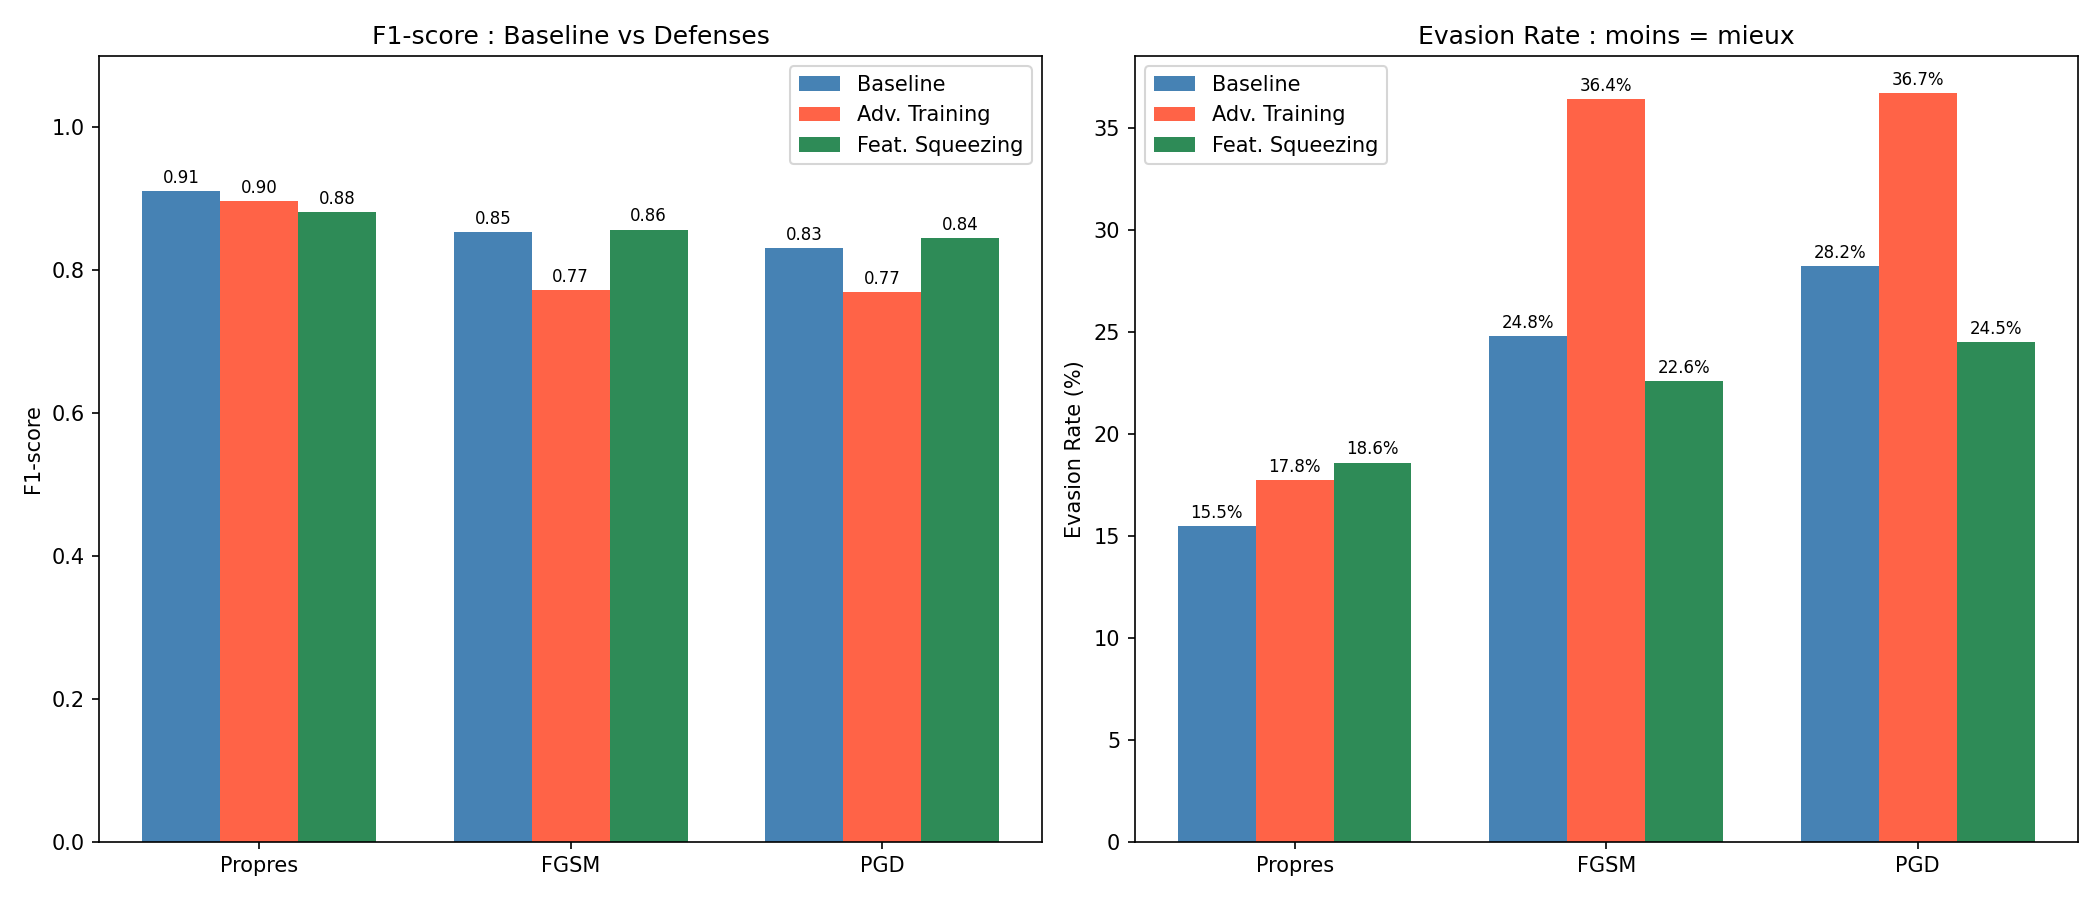
\includegraphics[width=\textwidth]{../results/final_comparison.png}
\end{frame}

\begin{frame}{Robustesse vs Budget $\varepsilon$}
\begin{columns}[T]
\column{0.54\textwidth}
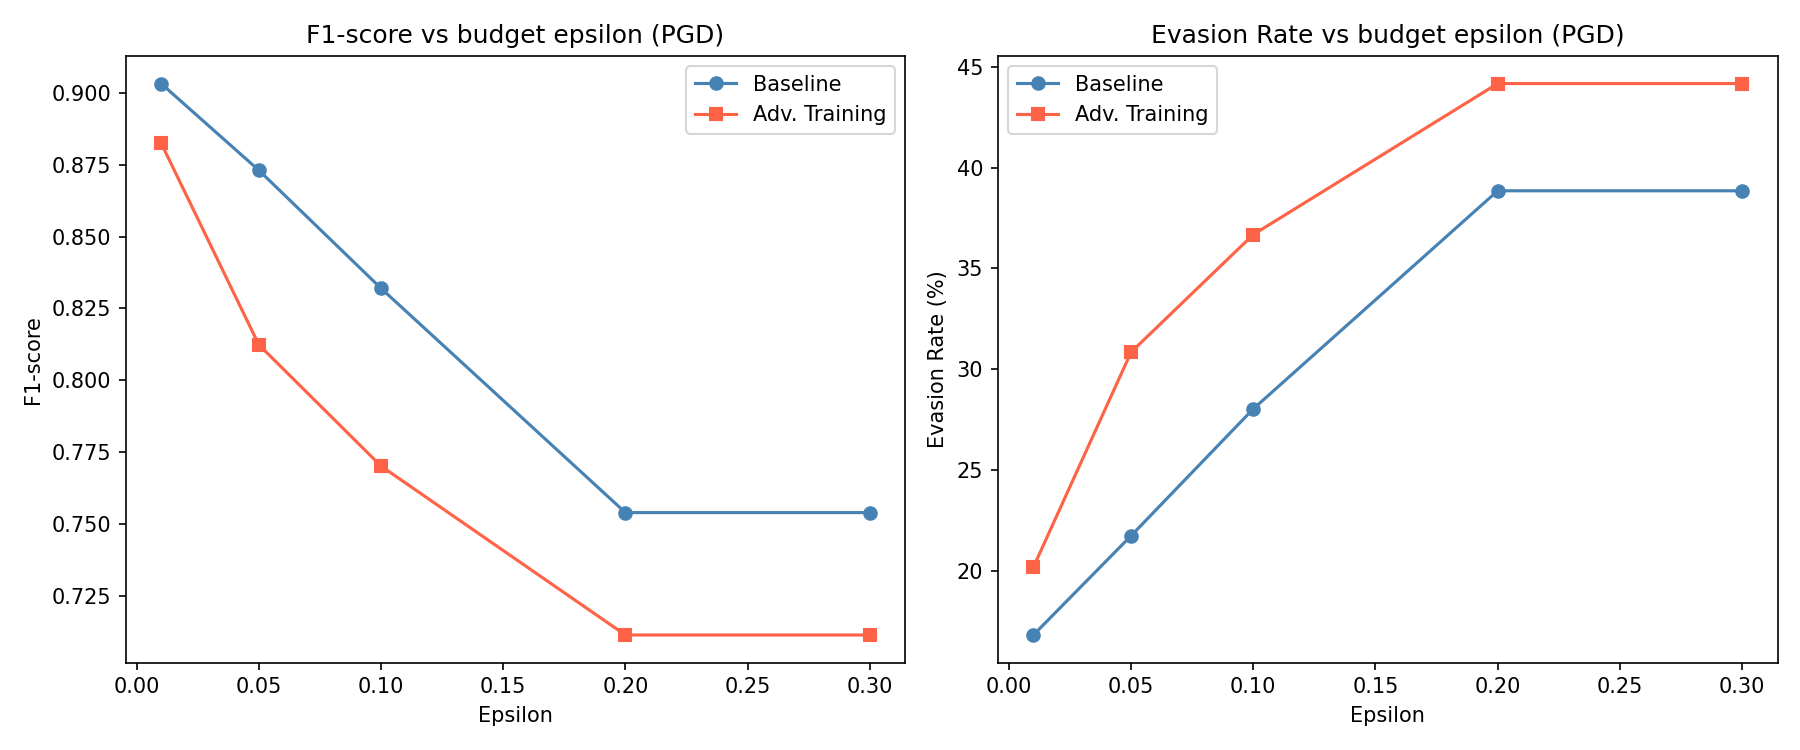
\includegraphics[width=\textwidth]{../results/robustness_vs_epsilon.png}

\column{0.44\textwidth}
\begin{table}
\scriptsize
\begin{tabular}{lrr}
\toprule
$\varepsilon$ & \textbf{Baseline} & \textbf{Adv. Train.} \\
\midrule
0.05 & 0.874 & 0.813 \\
0.10 & 0.840 & 0.774 \\
0.30 & 0.700 & 0.659 \\
\bottomrule
\end{tabular}
\end{table}
\vspace{0.4em}
\begin{itemize}
    \item Les deux mod\`eles se d\'egradent avec $\varepsilon$
    \item L'adversarial training (10 epochs seulement) est moins robuste ici
    \item Avec 30~epochs + PGD dans l'entra\^inement, les r\'esultats seraient meilleurs
\end{itemize}
\end{columns}
\end{frame}

\begin{frame}{Matrices de Confusion}
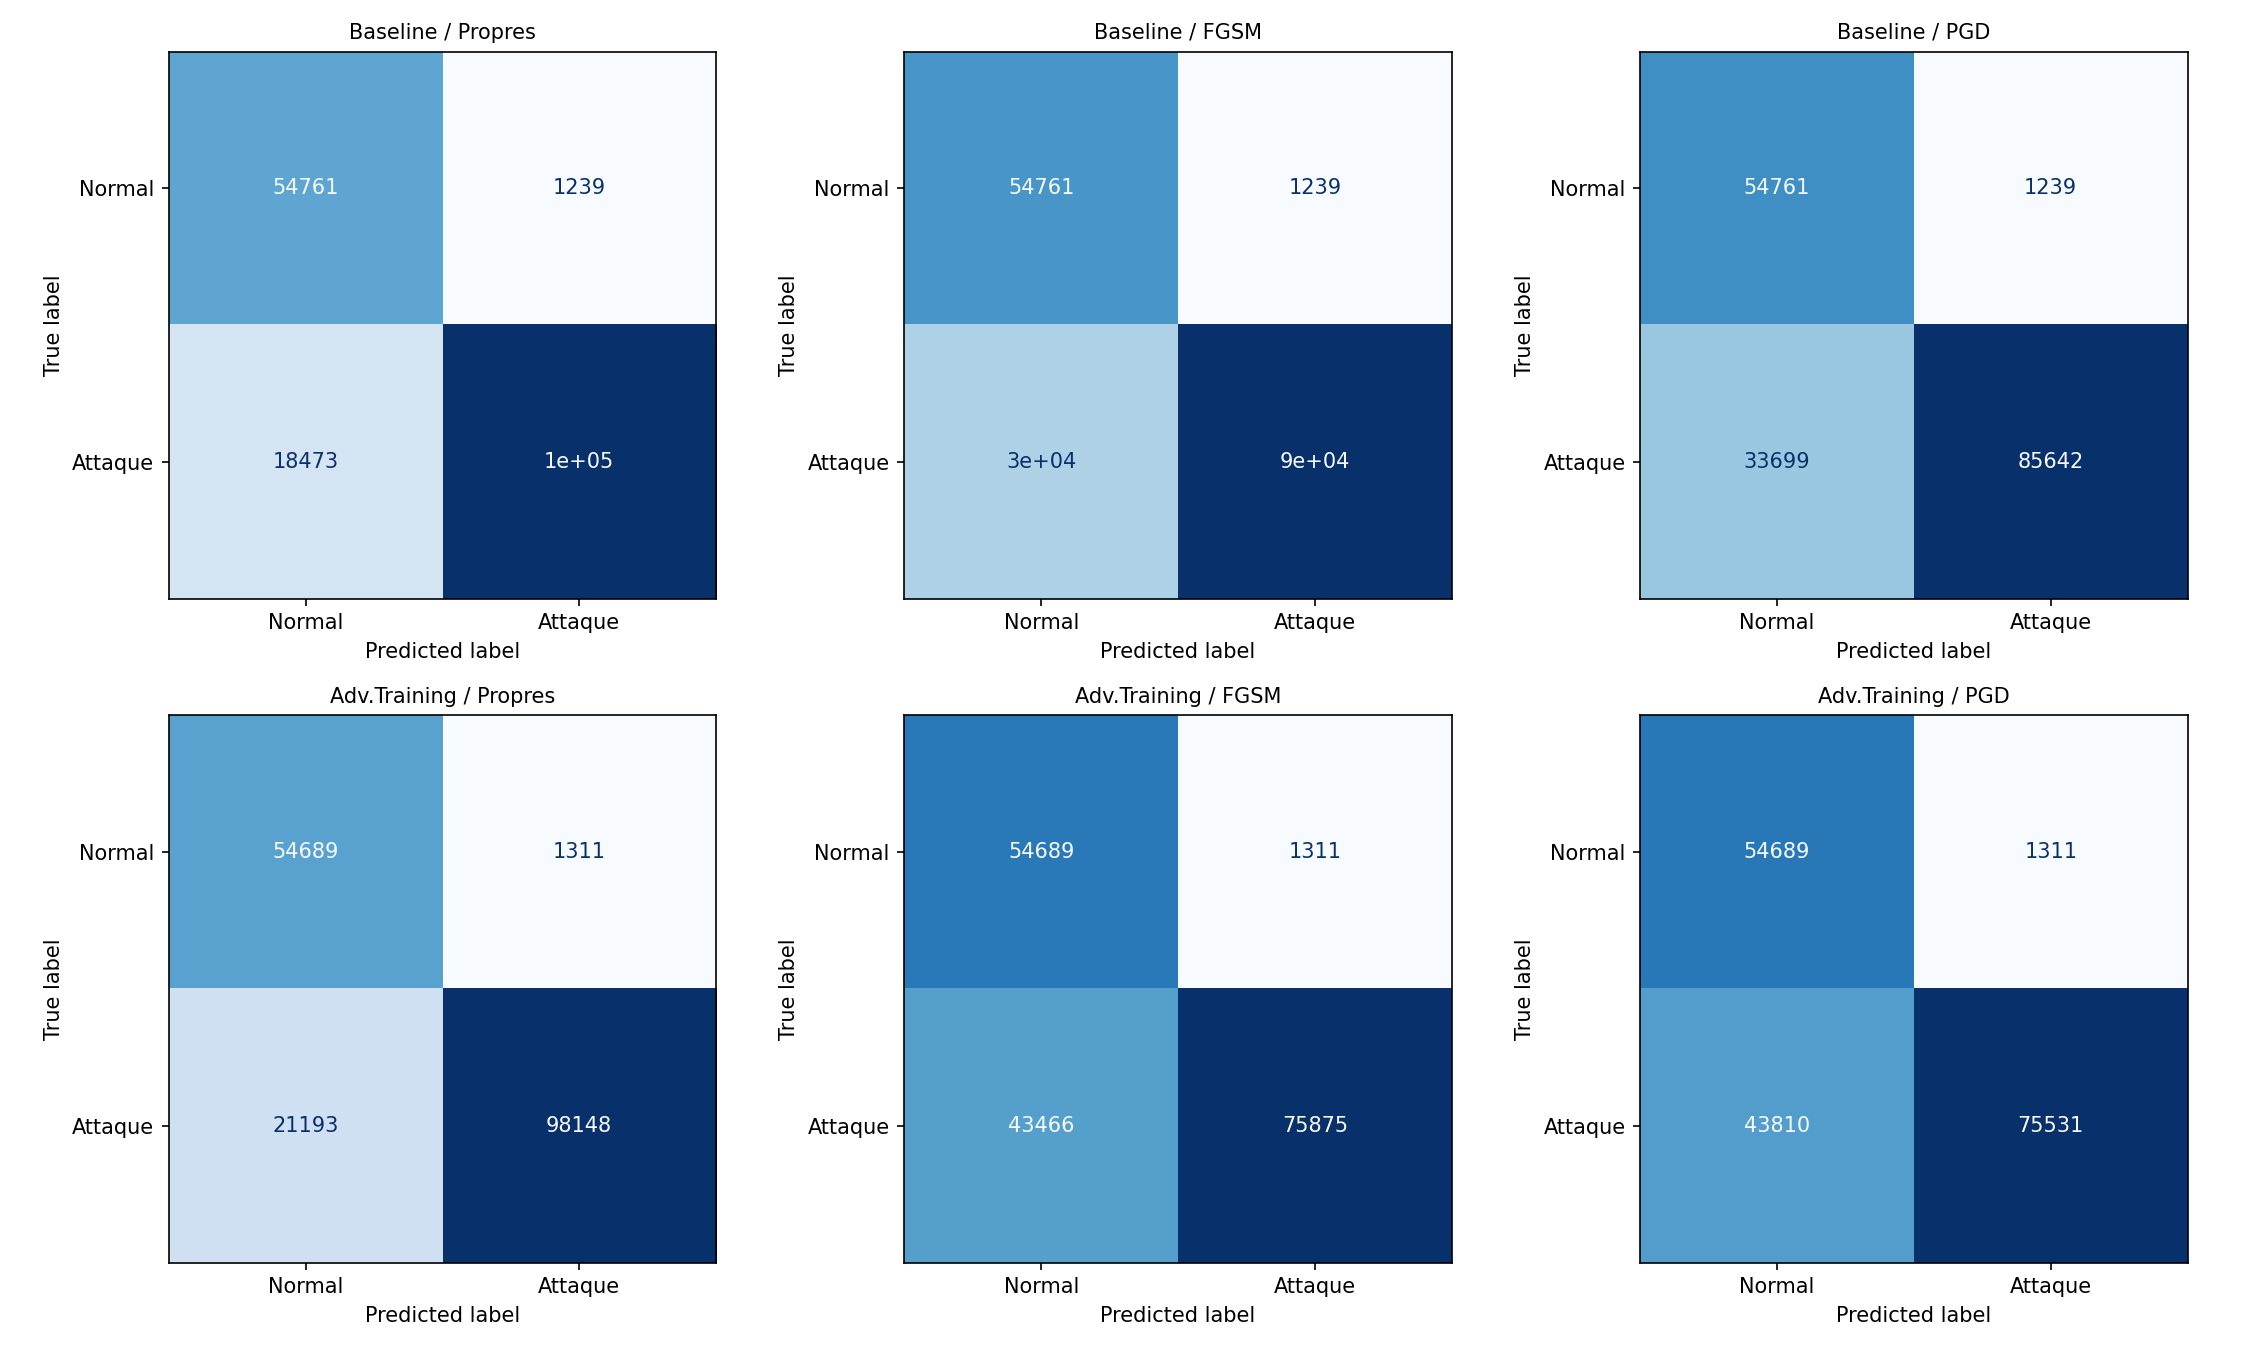
\includegraphics[width=\textwidth]{../results/confusion_matrices.png}
\end{frame}

%% ============================================================
\section{Conclusion}
%% ============================================================

\begin{frame}{Conclusion}
\begin{columns}[T]
\column{0.48\textwidth}
\begin{block}{Ce qu'on a montr\'e}
\begin{itemize}
    \item MLP baseline : F1 = \textbf{0.911}, evasion \textbf{15.5\%}
    \item FGSM/PGD font \'evader \textbf{28\%} des attaques
    \item Adversarial training (FGSM-AT, PGD-AT, PGD-AT corr.) : \alert{\'echec sur les 3 variantes} --- evasion 36--41.5\%
    \item \textbf{Feature Squeezing} : seule d\'efense efficace (evasion \textbf{24.5\%})
\end{itemize}
\end{block}

\column{0.48\textwidth}
\begin{alertblock}{Pourquoi l'adv. training \'echoue}
Les donn\'ees r\'eseau sont \textbf{tabulaires et h\'et\'erog\`enes} --- pas de structure spatiale.
Les 3 variantes souffrent respectivement de robustness gap, oubli catastrophique, et gradient masking.
\end{alertblock}

\vspace{0.3em}
\begin{exampleblock}{Perspectives}
\begin{itemize}
    \item Ratio propres/adversariaux calibr\'e
    \item AutoAttack pour \'evaluation plus robuste
    \item Randomized smoothing (certifi\'e)
\end{itemize}
\end{exampleblock}
\end{columns}
\end{frame}

\begin{frame}[plain]
\begin{center}
\vspace{2em}
{\LARGE\bfseries\color{myblue} Merci}\\[1em]
{\large Questions ?}\\[2em]
\begin{tabular}{ll}
\textbf{Dataset} & UNSW-NB15 (Moustafa \& Slay, 2015) \\
\textbf{FGSM}    & Goodfellow et al., ICLR 2015 \\
\textbf{PGD}     & Madry et al., ICLR 2018 \\
\textbf{Feat. Squeezing} & Xu et al., NDSS 2018 \\
\end{tabular}
\vspace{1.5em}

\footnotesize\color{gray}
Code : \texttt{github.com/zakeelm6/deep-learning-project-adversarial-IDS}
\end{center}
\end{frame}

\end{document}
